\subsubsection{Insertion Sort}

Figure \ref{fig:net_insertion_sort} illustrates the time it takes for each language, run in the .NET environment, to sort 10'000 randomly generated positive integers in ascending order.

\begin{figure}[h]
	\centering
	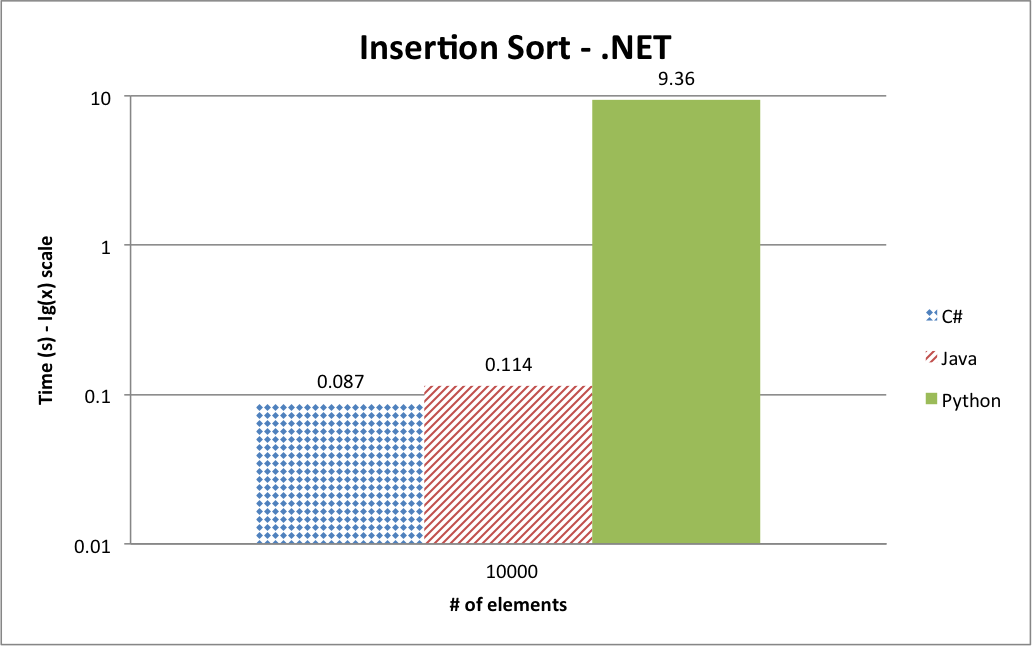
\includegraphics[width=1.0\linewidth]{chapters/new_media/InsertionSortNet.png}
	\caption{This test is run in the .NET environment and uses the Insertion sort algorithm to sort 10'000 elements in ascending order. Lower is better. Note that the vertical axis is base 10 logarithmic. C\# is the fastest with 0.087 seconds. Java is a close second with 0.114 seconds. Python is the worst with 9.36 seconds.}
	\label{fig:net_insertion_sort}
\end{figure}
